\chapter{Umsetzung und Ergebnisse}\label{ch:realization}

In diesem Kapitel wird die Umsetzung einer typischen Hybrid Cloud Anwendung betrachtet. 

Auf einem lokalen Rechner wird Spectrum Scale als Cluster-Speicher eingerichtet, was in diesem Aufbau den \gls{On Premise} Teil der Software darstellt.
In der öffentlichen Cloud von IBM (Bluemix) wird eine über das Internet zugängliche Anwendung zur Verfügung gestellt, die Zugriff auf die Daten des Clusters gewährt. Als Schnittstelle zwischen dieser Webanwendung und Spectrum Scale wird der \ac{COS} verwendet. Scale kann hier seine lokalen Daten über Cloud Sharing exportieren und neue, vom Nutzer erstellte Daten, importieren.

An dieser Stelle wird besonders Wert darauf gelegt, dass die beschrieben Schritte nachvollziehbar und nachbildbar dargestellt werden. Es wird also nicht nur ein Fokus auf die Ergebnisse gelegt, sondern auch auf die verwendeten Techniken.

\section{Aufsetzen einer Spectrum Scale Instanz in lokaler Umgebung}
Obwohl Spectrum Scale eigentlich dafür vorgesehen ist, auf multiplen Systemen installiert zu werden, ist es möglich ein minimales Setup mit zwei oder auch nur einer Maschine zu ermöglichen. Speziell für letzteren Fall gibt es ein von IBM zur Verfügung gestelltes Demoabbild.

Dies ist für ein Produktivsystem absolut nicht zu empfehlen, da aufgrund der verteilten Architektur von Scale ein hoher Leistungsmehraufwand auf einem einzelnen Rechner entsteht und kein Gewinn aus parallelem Dateizugriff gezogen werden kann.

Für diese Arbeit wird ein vorbereitetes Abbild verwendet, das bereits eine ältere Version von Cloud Tiering unterstützt.

\textbf{Vorbereitung der Host Maschine}\\
Im ersten Schritt muss auf dem zu verwendenden Rechner eine Virtualisierungslösung installiert werden. Es wurde sich hierbei für \ac{KVM} im Zusammenspiel mit \ac{QEMU} entschieden, da diese kostenlos verwendbar und in Linux integriert sind. 

Bei QEMU handelt es sich um einen Open Source virtuelle Maschinen Emulator und Virtualisierer mit nur geringem Leistungsverlust für das Gastsystem. Volle Virtualisierung durch direktes Ausführen der Gastbefehle auf der Gastgeber CPU kann aber nur in Zusammenarbeit mit einem Xen Hypervisor oder mit dem KVM Kernel Modul auf Linux Systemen erreicht werden \parencite{qemu.2017}. 
KVM ermöglicht Virtualisierung mithilfe von Intel/Amd CPUs der x86 Bauart, die so genannte virtuelle Erweiterungen zur Verfügung stellen. Es besteht aus einem ladbaren Kernel Modul, das eine grundsätzliche Infrastruktur für genannte Aufgaben zur Verfügung stellt \parencite{kvm.2017}.
Zusätzlich wird das Tool \textit{Virtual Manager} verwendet, das eine grafische Oberfläche für die \acs{VM}s zur Verfügung stellt.

Die komplette relevante Software ist über gebräuchliche Paketverwaltungssysteme verfügbar (Advanced Packaging Tool, Red Hat Package Manager). Eine beispielhafte Installation für Red Hat Linux, laufend auf einer x86 Intel CPU, kann so aussehen (Ein laufendes System mit installiertem X Server wird vorausgesetzt):\\ 

\begin{lstlisting}[language=bash, caption=Einrichtung von KVM und QEMU]
[root@host ~]# grep -E '(vmx|svm)' /proc/cpuinfo 

[root@host ~]# yum update
[root@host ~]# yum install qemu-kvm qemu-img virt-manager libvirt libvirt-python libvirt-client virt-install virt-viewer bridge-utils

[root@host ~]# systemctl start libvirtd
[root@host ~]# systemctl enable libvirtd

[root@host ~]# lsmod | grep kvm
kvm_intel             162153  0
kvm                   525409  1 kvm_intel
\end{lstlisting} 

Im obigen Beispiel wird zuerst überprüft, ob das System Hardware Virtualisierung unterstützt. Falls diese nicht vorhanden ist, kann KVM nicht verwendet werden, was zu einer massiven Verschlechterung der Leistung der VM führt.
Im nächsten Schritt wird zuerst die Paketliste aktualisiert, dann die notwendige Software installiert und ihr Service gestartet. Als letztes überprüft man, ob das KVM Module richtig geladen wurde, der Output zeigt das geladene Modul für Intel CPUs.

\textbf{Installation des Spectrum Scale Probeabbilds}\\
Das Probeabbild ist zum leichteren Umgang in vier einzelne .img Abbilder aufgeteilt worden. Zusätzlich hierzu gibt es drei XML Dateien, die zur Konfiguration der VM und der Einrichtung von notwendigen privaten Netzwerken dienen.

Das erste virtuelle Netzwerk reicht von 10.0.2.1 zu 10.0.2.254 und wird für die Kommunikation des \acs{NSD} Servers und des Daemon von Spectrum Scale benutzt. Das zweite (192.168.56.1 bis 192.168.56.254) wird verwendet, um das Administrations UI über das Web erreichbar zu machen.

Bei der Konfigurationsdatei für die VM (SpectrumScale423\_TrialVM\_TCT.xml) muss Imagedateipfad und die Bezeichnung der Maschine (auslesbar durch \textit{virsh capabilities}) angepasst werden, da diese OS spezifisch abweichen können. Die XML Dateien der virtuellen Netzwerke müssen nur angepasst werden, wenn die festgelegten IDs auf dem System bereits existieren: \\

\begin{lstlisting}[language=xml, caption=Veränderung der relevanten XML Konfiguration]
<domain type='kvm' xmlns:qemu='http://libvirt.org/schemas/domain/qemu/1.0'>
	<name>SpectrumScale423_TrialVM_TCT</name>
	...
	<os>
		<type arch='x86_64' machine='(*@\colorbox{yellow}{pc-i440fx-rhel7.0.0}@*)'>hvm</type> 
		<boot dev='hd'/>
	</os>
	...
	<devices>
		<emulator>/usr/libexec/qemu-kvm</emulator>
		<disk type='file' device='disk'>
			<driver name='qemu' type='raw'/>
			<source file='(*@\colorbox{yellow}{/home/simon/images/SpectrumScale421\_TrialVM-disk1.img}@*)'/>
			<target dev='hda' bus='ide'/>
			<address type='drive' controller='0' bus='0' target='0' unit='0'/>
		</disk>
		<disk type='file' device='disk'>
			<source file='(*@\colorbox{yellow}{/home/simon/images/SpectrumScale421\_TrialVM-disk2.img}@*)'/>
			...
		</disk>
		<disk type='file' device='disk'>
			<source file='(*@\colorbox{yellow}{/home/simon/images/SpectrumScale421\_TrialVM-disk3.img}@*)'/>
			...
		</disk>
		<disk type='file' device='disk'>
			<source file='(*@\colorbox{yellow}{/home/simon/images/SpectrumScale421\_TrialVM-disk4.img}@*)'/>
			...
		</disk>
	...
	</devices>
...
\end{lstlisting}

Diese grundsätzlicmhe Konfiguration nach individueller Anpassung kann wieder über diverse Bash Eingaben automatisiert werden: \\

\begin{lstlisting}[language=bash, caption=Portierung des VM Abbilds]
[root@host ~]# mkdir images && mv <your image files and xml configuration> images
[root@host ~]# virsh define SpectrumScale423_TrialVM_TCT.xml 

[root@host ~]# virsh net-define SpectrumScale_network1.xml
[root@host ~]# virsh net-define SpectrumScale_network2.xml

[root@host ~]# virt-manager
\end{lstlisting}

Die VM ist nun nach dem ersten Start vollständig aufgesetzt und die Administrationsoberfläche über die IP 192.168.56.101 zugänglich.

\textbf{Update des Spectrum Scale Systems}\\
Nach ersten Versuchen mit dem Spectrum Scale System Version 4.2.2.1 hat sich herausgestellt, dass das Cloud Tiering Feature nicht mit der öffentlichen Version von \acs{COS} kommunizieren kann. Die Verbindung kommt nicht zustande, da keine abweichende Endpunkt URL angenommen wird.

Deswegen muss zuerst die Version 4.2.3.1 installiert werden, um unser Hybrid Cloud Setup zu ermöglichen. Bei Spectrum Scale geschieht dies normalerweise ausgehend von einem Administrationsknoten, der dann die Updates über das gesamte Netz verteilt. Die Patchdatei wird mithilfe von \ac{SCP} von der Hostmaschine auf das, in dieser Konstellation bestehende, Gastsystem kopiert.	

Dort kann sie ausgeführt werden, wodurch sich das Installationstool \textit{spectrumscale} installiert. Nachdem man in diesem die Adressen der Knoten (hier der eigene), kann die Aktualisierung gestartet werden. Das Werkzeug ist hierbei selbst erklärend und führt durch die einzelnen Schritte, es werden auch entsprechende Hinweise für fehlende Konfigurationseingaben gegeben.
Im Laufe von dieser müssen eventuell der Cloud Service manuell gestoppt werden, sofern eine entsprechende Fehlermeldung angezeigt wird.

Nach erfolgreichen Update kann nun die Cloud Funktionalität konfiguriert werden.

\textbf{Installation Transparent Cloud Tiering}\\

Eine ausführliche Anleitung zum Installieren von Cloud Tiering Knoten auf einer einfachen Installation von Spectrum Scale ist in dieser Quelle beschrieben: \cite{mani.2017}.

In diesem Anwendungsfall ist die Installation nicht notwendig. Auf den eingerichteten VM-Abbildern ist der Clouddienst bereits funktionsfähig.



\section{Umsetzung des Cloud Tierings \& Implementierung der Hybrid Cloud Lösung}
Nach erfolgreicher Einrichtung einer Cloud Node im Spectrum Scale Cluster, kann diese nun mit unterschiedlichen Cloud Speichern verbunden werden.

Bei der Einrichtung wird davon ausgegangen, dass folgende Einstellungen vorgenommen wurden:
\begin{itemize}
	\item Name der NodeClass: \textbf{TCTNodeClass}
	\item Cloud Typ: \textbf{cleversafe-new}
	\item Cloud Bezeichnung: \textbf{mcstore}
	\item Name des Cloud-Dateisystems: \textbf{fs1}
\end{itemize}

Nach Hochfahren des Clusters kann mit \lstinline|mmhealth node show|, der Status der unterschiedlichen Dienste untersucht werden. Auf einer einzelnen Maschine kann es aber einige Minuten bauen, bis Scale vollständig hochgefahren ist.

Um den Zustand des Cloud Dienstes zu inspizieren, mit ihm zu arbeiten (Datei Sharing / Tiering) oder ihn zu verändern wird das \lstinline|mmcloudgateway| Programm verwendet. Falls dieser nicht automatisch beim Systemstart initialisiert wird, kann er mithilfe von \lstinline|mmcloudgateway service start -N TCTNodeClass| manuell gestartet werden.

\begin{figure}[hbt]
	\centering
	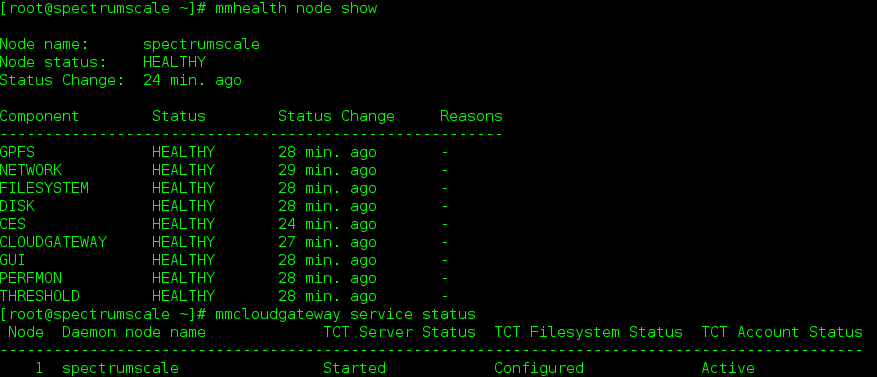
\includegraphics[scale=0.5]{images/scale-status}
	\caption{Beispielhafte Ausgabe von \lstinline|mmhealth| und \lstinline|mmcloudgateway| - mit konfiguriertem Cloudgateway}
	\label{fig:saclestatus}
\end{figure}


\textbf{Einrichtung des Cloud Sharing Accounts}\\
Nun muss zuerst die S3 Verbindung mit \ac{COS} hergestellt werden. Dafür sollte ein Test der Account Daten im Vorhinhein stattfinden, um spätere Probleme bei der Einrichtung verhindern.

Ein IBM Cloud Object Storage Account auf Softlayer kann unter dieser URL \url{https://www.ibm.com/cloud-computing/bluemix/cloud-object-storage} eingerichtet werden. 

Nach erfolgreicher Erstellung kann ein erster Bucket erstellt und Nutzername, Adresse des Endpunkts und Passwort ausgelesen werden. Hierbei gibt es Unterschiede bei der Befehl Syntax zwischen Spectrum Scale und \ac{COS}. 
Der Nutzername wird bei S3 kompatiblen Schnittstellen normalerweise als \textit{AccessKeyId} und das Passwort als \textit{SecretAccessKey} bezeichnet.\\

\begin{lstlisting}[language=bash, caption=Vortest des Cloud Sharing Accounts]
mmcloudgateway account pre-test --cloud-type cleversafe-new --username "<username>" --pwd-file <path/file/your/secretAccessKey> --cloud-url <cos/endpoint>
\end{lstlisting}

Nach Ausführung wird eine Testverbindung aufgebaut, entstehen keine Fehlermeldungen kann nun der Account eingerichtet werden. An dieser Stelle ist es extrem wichtig, dass die Option \lstinline|--enc-enable| auf \lstinline|FALSE| gesetzt wird. Ansonsten kann das beabsichtigte Cloud Sharing nicht umgesetzt werden, da beim Export eine Dateiverschlüsselung stattfindet. Diese macht das Lesen der Informationen von anderen Anwendungen (hier unsere Demoanwendung) unmöglich.

Die Befehlssyntax benötigt an dieser Stelle aber noch weitere Informationen, die für den Test nicht notwendig waren:\\

\begin{lstlisting}[language=bash, caption=Einrichtung des Cloud Sharing Accounts]
mmcloudgateway account create --cloud-nodeclass TCTNodeClass --cloud-name mcstore --cloud-type cleversafe-new --username "<username>" --pwd-file <path/file/your/secretAccessKey> --enable TRUE --cloud-url <cos/endpoint> --enc-enable FALSE
\end{lstlisting}

Nach erfolgreicher Ausführung des Befehls ist der Account fertig eingerichtet und man sollte folgende Ausgabe (\autoref{fig:saclestatus}) bei dem Überprüfen des Cloud Services sehen.

\textbf{Export von lokalen Dateien in die Cloud}\\
Um Informationen in den konfigurierten Cloud Account zu exportieren, muss zuerst in das ausgewählte Datei System für die Cloud Knoten gewechselt werden (hier: \lstinline|cd /gpfs/fs1|).

Mit dem bereits bekannten \lstinline|mmcloudgateway| Befehl können nun einzelne oder mehrere Dateien zwischen \ac{COS} und der lokalen Maschine kopiert werden.

Es besteht die Möglichkeit, Metadaten beim Sharing zu erhalten und alle exportierten Files in einem Manifest festzuhalten. Dieses hilft beim späteren Import, da eine Liste aller exportierten Dateien vorliegt. 

\begin{lstlisting}[language=bash, caption=Export von lokalen Dateien]
mmcloudgateway files export <path/to/file> --manifest-file manifest.txt --export-metadata
\end{lstlisting}

\begin{lstlisting}[language=bash, caption=Import von COS Dateien]
mmcloudgateway files import <fileKey> --import-metadata
\end{lstlisting}

Weitere Informationen hierzu befinden sich in \cite[S. 613]{scale.2017}.

\textbf{Erweiterung der Spectrum Scale Funktionalität}\\
Da Spectrum Scale keinerlei Kontrolle über die geteilten Daten hat, wird es auch nicht über mögliche neue Dateien informiert. Diese können also nativ nicht wieder importiert werden, da keine Informationen vorliegen.

Um dies zu umgehen, gibt es zwei Möglichkeiten: Es kann ein kleiner Webserver auf einem Spectrum Scale Knoten aufgesetzt werden, der von außen über Änderungen informiert wird und diese dann in das Manifest schreibt. Nachteil an dieser Lösung ist, dass zusätzliche Software für Scale entwicklet werden muss und diese auch immer nur auf einem Knoten läuft, was zu Leistungsengpässen führen kann.

Alternativ kann die Manifest Datei auch mit in den Cloudspeicher hochgeladen werden. Von hier kann eine Aktualisierung durch die Cloudanwendung (\autoref{sec:application}) geschehen, jedes Mal wenn neue Daten hinzugefügt werden. Spectrum Scale kann nun immer als erstes die Manifest Datei wieder importieren und bekommt mit dieser dann Information über die Dateiveränderung.

Offensichtlich ist zweite Lösung besser, da keine Veränderung am Cluster vorgenommen werden muss.

\section{Entwicklung der Bluemix Demoanwendung}
Das Szenario der \textit{CloudTieringDemo} zeigt, wie eine grafische webbasierte Schnittstelle für \ac{COS} erzeugt werden kann, die zusätzlich die Analyse von hoch geladenen Bildern ermöglicht. Das Aufsetzen des notwendigen Spectrum Scale Clustern wurde hierbei in den vorherigen Abschnitten beschrieben.
Dieser Teil der Beschreibung umfasst das Entwickeln der Cloudanwendung, Aufsetzen und Einrichten auf Bluemix mithilfe einer \ac{CD}-Pipeline und \gls{Git} zur Versionsverwaltung. Anhand dieses Beispieles sollen die Möglichkeit der Kombination verschiedener Dienste verdeutlicht und eine wiederverwendbare Architektur erzeugt werden. Diese kann dann in anderen Projekten als Schnellstart dienen.

\begin{center}
	\colorbox{gray}{\parbox{0.9\textwidth}{Der Code der Anwendung kann von GitLab heruntergeladen werden und steht öffentlich zur Verfügung: \url{https://git.ng.bluemix.net/simuelle/CloudTieringDemo}}}
\end{center}

\subsection{Architektur der Anwendung}
An dieser Stelle werden die wichtigsten Teile der Anwendung untersucht, visualisiert und in ein Verhältnis zueinander gestellt. Dafür werden Kontext-, Operations- und Klassendiagramme zur Verfügung gezeigt und erläutert.

Die auf Bluemix laufende Anwendung besteht aus mehreren Komponenten für Frontend und Backend. Auf der einen Seite gibt es einen auf Node.js basierenden Anwendungsserver, der die eigentliche Logik der Anwendung kapselt und mithilfe einer \gls{REST}-Schnittstelle verschiedene Dienste bereitstellt.

Wie in \autoref{fig:democontextdiagram} zu sehen ist, kommuniziert die Anwendung mit zwei externen Ressourcen. Eine von diesen ist der Spectrum Scale Cluster angebunden an den \ac{COS} mithilfe von Cloud Sharing und die andere ist die Deep Learning Software zur Bildanalyse von IBM Watson.

\begin{figure}[hbt]
	\centering
	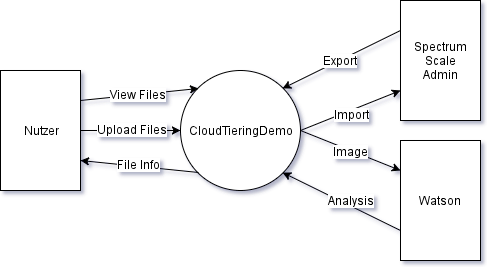
\includegraphics[scale=0.75]{images/demo-context-diagram}
	\caption{Kontextdiagramm der Demo}
	\label{fig:democontextdiagram}
\end{figure}

In \autoref{fig:demosequenzdiagram} sieht man eine typische Aktionssequenz, ausgelöst durch einen Nutzeraktion. Der hier dargestellte Hochladeprozess kann stellvertretend für alle Aktionen zwischen Client (Internetbrowser des Nutzers) und \ac{COS} betrachtet werden.
Zuerst wird ein asynchroner Request an den Node.js Applikationsserver gestellt, dieser erzeugt einen Request für den \ac{COS}-Server und sendet danach die Daten bzw. eine Bestätigung des Uploads an den Nutzer.
Beim Scheitern der Anfrage wird eine entsprechende Fehlermeldung an den Browser gesendet.

\begin{figure}[hbt]
	\centering
	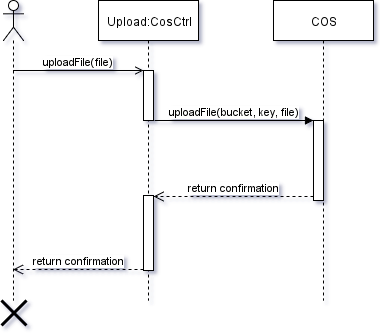
\includegraphics[scale=0.85]{images/demo-sequenz-diagram}
	\caption{Sequenz-Diagramm des Hochladeprozesses in der Demo}
	\label{fig:demosequenzdiagram}
\end{figure}

Ein Spezialfall stellt hierbei die Bildanalyse durch den Watsondienst dar (\autoref{fig:demosequenzdiagramwatson}). Das ausgewählte Bild muss erst akquiriert werden und wird dann zum Visual Recognition-Server hochgeladen. Nachdem dieser entsprechende Metadaten für die Bilddatei erzeugt hat, werden sie ebenfalls im Cloudspeicher abgelegt und eine Bestätigung an den Nutzer gesendet.
Diese kann einige ausgewählte Erkenntnisse über die Datei enthalten.

\begin{figure}[hbt]
	\centering
	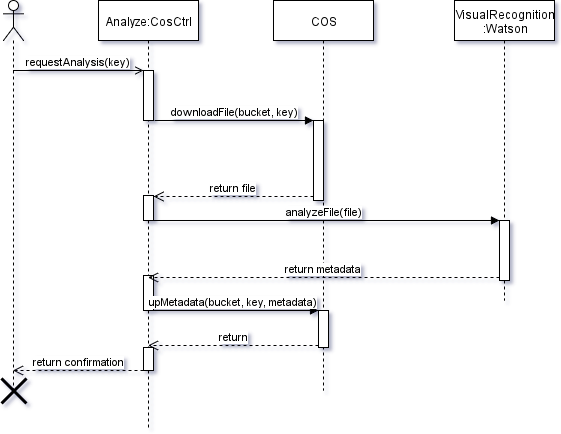
\includegraphics[scale=0.75]{images/demo-sequenz-diagram-watson}
	\caption{Sequenz-Diagramm der Bildanalyse mit Watson in der Demo}
	\label{fig:demosequenzdiagramwatson}
\end{figure}

\textbf{Backend}\\
Der mit Node.js und Express laufende Server implementiert eine leicht abgeändertes \ac{MVC} Framework. Betrachtet man die Ordnerstruktur repräsentiert diese die einzelnen Bestandteile des Entwicklungsmusters.

\begin{itemize}
	\item \textbf{app.js}:\\
	Die Hauptdatei des Servers, die beim Starten ausgeführt wird. Hier werden notwendige Pakete initialisiert, weitergereicht und der Webserver konfiguriert.
	\item \textbf{controller/}:\\
	Die REST-Controller der Anwendung. Werden ausgeführt, wenn bestimmte ULRs aufgerufen wurden und delegieren Aufgaben an die Anwendungslogik. Sie übernehmen die gesamte Kommunikation mit der Frontendanwendung (Auslieferung von HTML-Inhalten oder REST-Antworten) und sorgen für eine einheitliche Formatierung der Antworten.
	\item \textbf{services/}:\\
	An dieser Stelle findet die gesamte Anwendungslogik und Datenmodellveränderung statt. Anfragen an \ac{COS} für den Datenaustausch starten hier, ebenso wie die Kommunikation mit anderen Diensten.
	Dedizierte Service Klassen können an jeden Controller übergeben werden und sind somit an verschiedenen Stelle der Anwendung benutzbar.
	\item \textbf{views/ und public/}:\\
	Im \textit{views/-Ordner} liegen alle Vorlagen für die HTML-Inhalte zur Auslieferung an das Frontend. Da im \ac{UI} auch Logik und Styling verwendet werden soll, liegen alle, von den HTML-Seiten verwendeten Skripte und Stylesheets, im \textit{public/-Ordner}.
	Diese sind aufgeteilt in Javascript-, CSS- und Bilddateien.
	\item \textbf{Sonstige Ordner und Dateien}:\\
	Zusätzlich gibt es noch eine Paketbeschreibung (\autoref{tab:npmpackages}) in der \textit{package.json} mit dem \textit{node\_modules/-Ordner} für die tatsächlichen Module und einen \textit{config/-Verzeichnis} für Einstellungen der Anwendung. Für das temporäre Speichern von Dateien wird der \textit{file\_cache/-Ordner} verwendet.
\end{itemize}

In der Implementierungsbeschreibung wird das Aufsetzen einer typischen Ablaufsequenz, inklusive aller anzupassenden Dateien, demonstriert.\\

\textbf{Frontend}\\
Wie oben beschrieben, existieren ebenfalls einige Dateien für das Frontend. Sie sorgen dafür, dass eine dynamische, anpassungsfähige und ästhetische Benutzung des Interface möglich ist.

Dies setzt natürlich auch eine gewisse Architektur voraus, die eine leichte Erweiterbarkeit ermöglicht. Somit liegt im Frontend folgende Ordnerstruktur vor:

\begin{itemize}
	\item \textbf{views/}: Die HTML-Vorlagen für die einzelnen Seiten der Anwendung
	\item \textbf{public/}
	\begin{itemize}
		\item \textbf{css/}:\\
		Hier liegt ein generelles Stylesheet (\textit{style.css}) für alle Seiten und spezialisierte Dateien für jede einzelne View.
		\item \textbf{img/}:\\
		Ein Speicherort für alle Bilddateien, die im Frontend verwendet werden
		\item \textbf{js/}:\\
		Das Wurzelverzeichnis für alle Javascriptdateien, die für die Logik der \ac{UI} benutzt werden. Auf der obersten Eben liegen dedizierte Skripts, die beim Ausführen der Seite ausgeführt werden.
		\begin{itemize}
			\item \textbf{controller/}:\\
			Controller, die Veränderung an der HTML-Datei auslösen und dynamische Änderungen, ohne Neuladen der Seite, erzeugen können 
			\item \textbf{services/}:\\
			Bestimmte Dienste sind hier angelegt, zum Beispiel die \gls{AJAX}-Kommunikation mit dem Backend. Sie sind von überall erreichbar und bieten verschiedene statische Methoden. Vergleichbar mit den serverseitigen Services.
		\end{itemize}
	\end{itemize}
\end{itemize}

Das Frontend spielt in dieser Anwendung eine untergeordnete Rolle (im Sinne eines schwachen Klienten) und es wird auch bei der Implementierungsbeschreibung hauptsächlich Wert auf die Serverstrukturen gelegt. Theoretisch kann die bestehende \ac{UI} leicht durch eine andere ausgewechselt werden, da nur eine lose Kopplung durch die \gls{REST}-API besteht.

\subsection{Implementierung}

Bevor die Implementierung gestartet werden kann, sollten einige Grundvoraussetzungen erfüllt sein:

\begin{itemize}
	\item Softlayer Cloud Object Storage Account mit S3-API(IBM COS)
	\item IBM Bluemix Account
	\item IBM Bluemix Kommandozeilen Werkzeug
	\item Node.js Version > 6.0.0
	\item \gls{Git}
\end{itemize}

Um diese Voraussetzungen zu erreichen, existiert eine umfangreiche Dokumentation in folgender Quelle: \cite[S. 129]{Rios.2017}.

An dieser Stelle wird nur grob auf das Setup eingegangen und mehr auf die eigentliche Implementierung fokussiert.

Nach erfolgreichen Anlegen der Benutzeraccounts und Installation der lokalen Tools, kann die Cloud Foundry-Anwendung angelegt werden. Hierzu muss zuerst die Anmeldung auf Bluemix erfolgen und die Navigation auf das Dashboard. Hier können neue Applikationen erzeugt werden. In unserem Anwendungsfall wird die Node.js Laufzeit Umgebung erzeugt, es muss nur ein eindeutiger Name für die App und die URL-Route ausgewählt werden.

Innerhalb weniger Momente sollte eine einfache Basisanwendung erreichbar sein. Um den Quellcode bearbeiten zu können, kann dieser entweder mit dem Bluemix Kommandozeilen Tool heruntergeladen oder ein Git-Verzeichnis erzeugt werden. Zweites ist wesentlich mächtiger, da sowohl eine vollständige Versionsverwaltung wie auch eine \ac{CD}-Pipeline zur Verfügung steht. Um sie zu erzeugen, muss im Dashboard die neue Anwendung ausgewählt und eine neue Toolchain erstellt werden. Es steht nun eine GitLab Umgebung und eine Standard konfigurierte Pipeline zur Verfügung.

Durch die normale Einstellung der Toolchain werden automatisch Git-Commits auf den \textit{master}-Zweig auf Bluemix deployed. Wenn ein Projekt mehreren Beitragenden hat, sollte dieses Verhalten verändert werden.

Mithilfe von \gls{Git} kann nun der Starter-Code heruntergeladen und für diesen Nutzungsfall angepasst werden.

Zuerst sollte die oben beschriebene Ordnerstruktur erzeugt und alle NPM-Abhängigkeiten installiert werden:

\begin{lstlisting}[language=bash, caption=Paket Installation und package.json erzeugung]
npm install aws-sdk body-parser bootstrap cfenv ejs express filesize jquery moment morgan multer promise toastr watson-developer-cloud --save
\end{lstlisting}

Die Anwendung lässt sich lokal zum Testen mit \lstinline|npm start| oder \lstinline|node app.js| starten.
 
Danach kann die \textit{app.js} angepasst werden, um den Grundstein für erste Routen und Seiten zu legen. An dieser Stelle wird eine gekürzte Version gezeigt, die nur den generellen Aufbau beleuchten soll.

\begin{lstlisting}[language=JavaScript, caption=Anpassung der Hauptdatei der Anwendung]
// DEPENDENCIES
const express = require('express');
... 
// EXPRESS SETUP
let app = express();
...
//STATIC FILE SERVING
app.use(express.static(__dirname + '/public'));
app.use(express.static(__dirname + '/file_cache'));
app.use('/bootstrap', express.static(__dirname + '/node_modules/bootstrap/dist'));
app.use('/jquery', express.static(__dirname + '/node_modules/jquery/dist'));
...
//VIEW ENGINE
app.set('view engine', 'ejs');
app.set('views',__dirname + '/views');

//SERVICES
const cosService = require('./services/cosService')(config);
...
//ROUTING
app.use('/api/v1', require('./controller/cosCtrl')(cosService, upload));
app.use('/', require('./controller/viewCtrl')());

//SERVER SETUP
app.listen(cfenv.getAppEnv().port, '0.0.0.0', function() { ... });
\end{lstlisting}

Im ersten Teil werden alle Abhängigkeiten der Anwendung geladen. Dies ist wichtig, damit keine mehrfache Initialisierung von bestimmten Modulen in der Anwendung stattfindet. Im nächsten Teil wird express mit verschiedener Middleware kombiniert und die statischen Ordner für Dateiauslieferung definiert. Für diese agiert express dann wie ein klassischer Dateiserver.
Im nächsten Schritt werden alle vom Nutzer definierten Dienste erstellt. Diese können dann im nächsten Abschnitt an die Controller weitergereicht werden, sofern Bedarf besteht.
Es gibt genau einen \lstinline|viewCtrl|, der zur Auslieferung der HTML-Vorlagen verwendet wird. Für jede neue Seite der \ac{UI} muss hier eine weitere GET-Route angelegt werden, die aus dem korrespondierenden EJS-Template das HTML generiert.
EJS ist hierbei ein Vorlagensprache, die Inline-Javascript ermöglicht und die Erzeugung von HTML-Seiten erleichtert.

Alle anderen Controller dienen zum Definieren der REST-Schnittstelle der Anwendung (zum Beispiel der \lstinline|cosCtrl|). Im letzten Teil der \textit{app.js} wird der HTTP-Server gestartet und aus den Bluemix-Umgebungsvariabeln der Port ausgelesen. Lokal wird hierbei einfach ein freier Port verwendet.\\

\textbf{Erzeugung eine REST-Schnittstellen Funktion}\\
An dieser Stelle betrachten wir die Implementierung der REST-Schnittstelle zum Löschen von Dokumenten in der \ac{COS}-Dateispeichersystem. Dieses kann als exemplarisch betrachtet werden, da nach den gleichen Entwicklungsmuster auch alle anderen API-Funktionen der Anwendung umgesetzt wurden. 

An erster Stelle muss der Controller erstellt werden, hierfür wird die Router Middleware von express verwendet. Mithilfe von dieser können logisch zusammenhängende URL-Routen innerhalb einzelner Module gegliedert werden. Das Löschen von Objekten wird hier in den \lstinline|CosCtrl| eingeordnet, der sämtliche direkte Interaktionen mit dem Dateispeicher verwaltet:\\

\begin{lstlisting}[language=JavaScript, caption=CosCtrl.js mit einer Route zur Dateilöschung]
const express = require('express');
const router = express.Router();

module.exports = function(cosService) {

	router.delete('/files/:id*', function(req, res) {
		let id = req.params.id + req.params[0];

		cosService.removeFile(id).done(function(data) {
			let response = {msg: 'File delete successful', delete: data};
			res.json(response);
		},
		function(err) {
			res.status(500).send(err);
		});
	});

	return router;
}
\end{lstlisting}

In den ersten beiden Zeilen wird der hier verwendete Router importiert. Zeile 3 definiert die Initalisierungsfunktion des Moduls, indem auch der hier verwendete \lstinline|cosService| übergeben wird.

Der nächste Block definiert nun die eigentliche Route: Diese verarbeitet nur DELETE HTTP Anfragen, die auf eine spezielle Route gemappt werden. Sofern die Basis-URL übereinstimmt, wird jeder Dateischlüssel (\lstinline|:id*|) angenommen. Der Schlüssel wird als nächstes ausgelesen und die entsprechende Servicefunktion übergeben. Deren Funktionsweise wird nach diesem Controller erklärt.

Da \gls{Promise}s Verwendung finden, kann eine der beiden definierten Funktionen, abhängig vom Ergebnis des Nutzerdienstes, aufgerufen werden. Die erste erzeugt eine Antwort für den Klienten und übergibt die Bestätigung von \ac{COS}. Im Fehlerfall wird ein HTTP Errorcode und der entstandene Fehler zurückgesendet.

Um das Modul nutzbar zu machen, muss jetzt nur noch der Service definiert werden:\\

\begin{lstlisting}[language=JavaScript, caption=CosService.js für die Kommunikation mit IBM COS]
const Promise = require('promise');
const aws = require('aws-sdk');

module.exports = function(config) {
	this.config = config;
	aws.config.loadFromPath(__dirname + '/../config/aws.json');
	this.ep = new aws.Endpoint(config.cos.endpoint);
	this.s3 = new aws.S3({ endpoint: this.ep });
	this.bucket = config.cos.bucket;
	
	this.removeFile = function(key) {
		return new Promise(function(fulfill, reject) {
			let params = {Bucket: this.bucket, Key: key};
			this.s3.deleteObject(params, function(err, data) {
				if(err) {
					reject(err);
				} else {
					fulfill(data);
				}
			});
		});
	};
	return this;
}
\end{lstlisting}

Zu Beginn werden wieder notwendige externe Module importiert und die Initialisierungsfunktion definiert. Informationen über Authentifizierung für \ac{COS} werden in der \lstinline|config| zentral von der Hauptdatei, welche aus dem globalen Konfigurationsfile \lstinline|config/config.js| liest, übergeben.

Mithilfe dieser wird der \ac{S3}-Klient und der richtige Bucket für die Anwendung erzeugt. 

In der eigentlich Funktion wird ein Promise-Wrapper erzeugt zum Ansprechen der relevante S3-API. Das Ergebnis wird über die Promise-Funktionen zurückgegeben.

Als letztes müssen nun nur noch der Service in der \lstinline|app.js| erstellt werden und an den Router übergeben. Danach kann der gestartete Server mit der neuen REST-URL angesprochen werden:\\

\begin{lstlisting}[language=JavaScript, caption=Einbindung der neuen Route in der app.js]
const cosService = require('./services/cosService')(config);
app.use('/api/v1', require('./controller/cosCtrl')(cosService));
\end{lstlisting}

\textbf{Erzeugung einer Frontend-Seite mit Backend Anbindung über AJAX}\\
Für die graphische Repräsentation existiert ebenfalls ein Arbeitsablauf: Zuerst muss eine EJS-Vorlage erstellt werden. Bei dieser handelt es sich, um eine erweiterte HTML-Datei. Es können, ähnlich wie bei PHP, andere Dateien (hier ein Header) eingebunden und die Sprache mit dynamischen Variablen erweitert werden.

Die neue Route muss im \lstinline|ViewCtrl| des Backends festgelegt werden:\\

\begin{lstlisting}[language=JavaScript, caption=Definition einer neuen Frontendroute in der viewCtrl.js]
router.get('/file/', function (req, res) {
	res.render('fileUpload');
});
\end{lstlisting}

An dieser Stelle kann man sehen, wie beim Ansprechen der URL eine neue HTML-Seite aus dem EJS-Template mit der \lstinline|render|-Funktion von express generiert wird.

Für jede Seite im Frontend gibt es eine eigenen CSS-Style, eine Initialisierungsdatei und einen Controller, der Veränderungen vornimmt. Diese Dateien werden statisch aus dem \lstinline|public/|-Verzeichnis ausgeliefert.

Das Erstellen der Seite zum Hochladen von Dateien wird hier als Beispiel untersucht und einige Codebeispiele betrachtet: \\

\begin{lstlisting}[language=JavaScript, caption=Initalisierungsfunktion der Uploadseite in der fileUpload.js]
let ctrl = null;
let main = function() {
	ctrl = new FileUploadCtrl();
};

let submitFile = function() {
	...
};

$( document ).ready(main);
\end{lstlisting}

Nachdem das Dokument geladen wurde wird zuerst die \lstinline|main|-Funktion ausgeführt und der Controller für die Seite erstellt. Die hier angedeutete \lstinline|submitFile|-Routine sendet einen POST-Request zum Server mit der angehängten Datei. Beim Erfolg der Routine gibt der \lstinline|FileUploadCtrl| ein positives Feedback im Frontend:\\

\begin{lstlisting}[language=JavaScript, caption=Initalisierungsfunktion der Uploadseite in der fileUpload.js]
class FileUploadCtrl {
	constructor() {
		$("#tabs>li.active").removeClass("active");
		$("#fileUploadTab").addClass("active");
		$("#reload-btn").hide();
	}

	uploadSuccess(result) {
		toastr.success('File upload successfull');
	}

	uploadError(error) {
		toastr.error('File upload failed');
	}
}        
\end{lstlisting}

Hier wird ein Toast erzeugt für den Erfolgs- oder Fehlerfall. Bei Erzeugung des Controllers wird die Navigation aktualisiert und der Tab auf aktiv gesetzt.

Bei anderen Seiten werden auch Services verwendet, die aber ungefähr den selben Aufbau, wie im Backend besitzen und hier nicht genauer erwähnt werden müssen. Sie stellen nur eine weitere Schicht, um die JQuery \gls{AJAX}-Schnittstelle dar.

\section{Ergebnisbetrachtung}
Ergebnis der experimentellen Hybrid-Cloud Aufstellung ist ein speziell konfigurierter Spectrum Scale Speichercluster mit Anbindungen an den \ac{COS} und eine neu entwickeltet Cloudanwendung mit Verbindung zu dem Objektspeicher und einem exemplarischen Analysedienst für Imagedateien.
Das aktuelle Setup ist ein VM-Abbild, das auch auf einer einzelnen Maschinen für Demozwecke verwendet werden kann.

Der Austausch von Daten zwischen Cluster und Cloud finden problemlos statt. Es muss nur darauf geachtet werden, dass keine Verschlüsselung beim Sharing stattfindet.

Einzige Schwierigkeit ist die Aktualisierung der Dateiliste auf der Seite von Spectrum Scale, da keine Funktion hierfür vorgesehen ist. Zur Lösung dieses Problems wird eine, alle vom Cluster exportieren Dateien enthaltende, Manifestdatei von Scale angelegt und in den Cloudspeicher hochgeladen. Die Demoanwendung kann nun diese Liste selber aktualisieren. Beim Importieren beginnt Scale mit dieser Manifestdatei und kann, anhand von ihr, alle anderen neuen Dateien herunterladen.

Die Demo stellt eine graphische Schnittstelle zum Speichern, Ansehen und Analysieren von Bilddateien und ist über IBM Bluemix erreichbar. Sie wird von einem express Server präsentiert, der ebenfalls eine einfache REST-API zum verwenden der oben beschriebenen Funktionen bereitstellt. Für die Bildanalyse wird IBM Watson Image Recognition verwendet, ein Dienst der mithilfe von Deep Learning Bilder klassifizieren kann.

Insgesamt funktioniert der Aufbau sehr gut und eine hohe Performanz wird bei einzelnen Anfragen geliefert, sodass sich das Szenario ausgezeichnet für Demozwecke verwendet werden kann.